% Generated by code/scripts/report_figures.py at 2026-11-03T07:57:50Z; do not edit.
% Inputs: artifacts/local/runs/pipeline-e2e-20261103T075711Z/run
\begin{figure}[t]
\centering
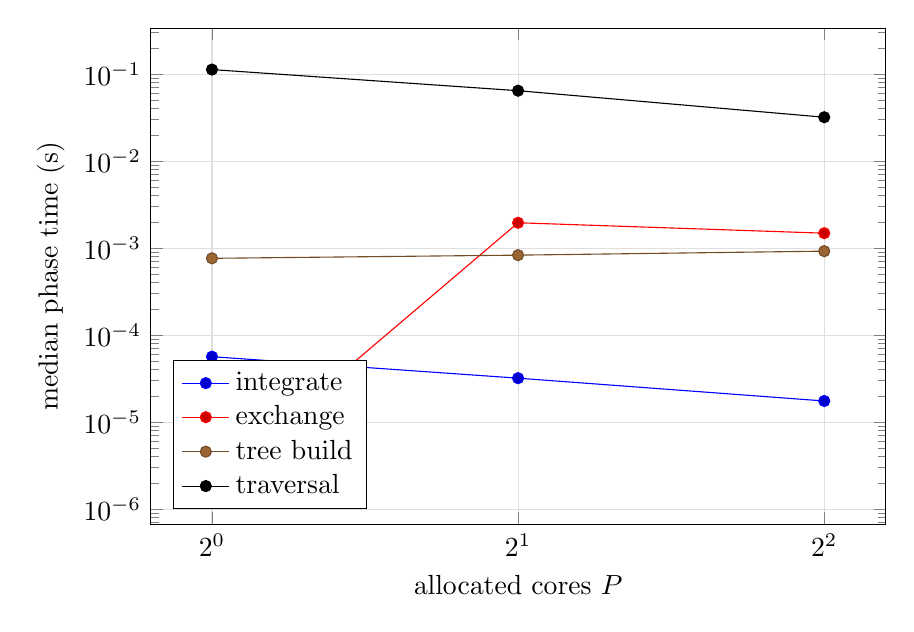
\begin{tikzpicture}
\begin{axis}[width=0.9\columnwidth, height=0.65\columnwidth, xlabel={allocated cores $P$}, ylabel={median phase time (s)}, xmode=log, log basis x=2, ymode=log, legend pos=south west, legend cell align=left, grid=major, grid style={gray!25}]
\addplot+[mark=*] coordinates {(1,5.65e-05) (2,3.2e-05) (4,1.75e-05)};
\addlegendentry{integrate}
\addplot+[mark=*] coordinates {(1,2e-06) (2,0.001956) (4,0.001484)};
\addlegendentry{exchange}
\addplot+[mark=*] coordinates {(1,0.0007635) (2,0.00083) (4,0.0009225)};
\addlegendentry{tree build}
\addplot+[mark=*] coordinates {(1,0.1127) (2,0.06443) (4,0.03193)};
\addlegendentry{traversal}
\end{axis}
\end{tikzpicture}
\caption{\textbf{LOCAL PIPELINE TEST, NOT A MEASUREMENT.} Phase times of the strong-scaling runs with $T=1$. Each phase is the maximum over ranks, so the phases need not sum to the wall time; zero values are omitted from the log axis.}
\label{fig:phases}
\end{figure}
